\documentclass[]{article}
\usepackage{polski} 
\usepackage[utf8]{inputenc}

% Listingi
\usepackage{listings}
\usepackage{xcolor}
\lstdefinestyle{sharpc}{language=[Sharp]C, frame=lr, rulecolor=\color{blue!80!black}}
\lstset{style=sharpc}

% interlinia, marginesy
\usepackage{geometry}
\newgeometry{tmargin=3cm, bmargin=3cm, lmargin=3.5cm, rmargin=3.5cm}
\linespread{1.25}

% obrazki
\usepackage{graphicx}
\graphicspath{ {./figures/} }
\usepackage{float}
\usepackage{subfig}


%opening
\title{Aplikacja webowa do obsługi planu zajęć}
\author{Paweł Nowak}

\begin{document}

\maketitle
\tableofcontents

\newpage
\section*{Wstęp}
Celem projektu było stworzenie aplikacji MVC w technologii .NET, która umożliwia przeglądanie oraz modyfikowanie planu zajęć akademickich. 

\section{Opis elementów projektu}
\subsection{Modele danych}
W projekcie uwzględniono trzy podstawowe modele danych:
\begin{itemize}
	\item \textbf{Group}, reprezentujący daną grupę studentów (np. Informatyka 1)
	\item \textbf{Lecturer}, reprezentujący prowadzącego
	\item \textbf{Lesson}, reprezentujący konkretny blok zajęciowy
\end{itemize}

\subsubsection{Group}
Zadaniem klasy $Group$ jest przechowywanie informacji na temat poszczególnych grup zajęciowych.
\begin{lstlisting}
public class Group
{
    public int ID { get; set; }
    public string Name { get; set; }
}
\end{lstlisting}
Parametr $ID$ jest unikalnym identyfikatorem każdej grupy, natomiast parametr $Name$ jest nazwą konkretnej grupy, np. $Informatyka 1$.

\subsubsection{Lecturer}
Zadaniem klasy $Lecturer$ jest przechowywanie danych na temat każdego prowadzącego.
\begin{lstlisting}
public class Lecturer
{
    public int ID { get; set; }
    public string FirstName { get; set; }
    public string SecondName { get; set; }
    public string Title { get; set; }
}
\end{lstlisting}
Poprzez $ID$ rozumie się unikalny identyfikator prowadzącego, $FirstName$ oraz $SecondName$ - imię oraz nazwisko, a $Title$ - tytuł naukowy.

\subsubsection{Lesson}
Klasa $Lesson$ umożliwia przechowywanie informacji o konkretnych zajęciach realizowanych na uczelni.
\begin{lstlisting}
public class Lesson
{
    public int ID { get; set; }
    public int GroupID { get; set; }
    public string Name { get; set; }
    public int LecturerID { get; set; }
    public DateTime StartTime { get; set; }
    public DateTime EndTime { get; set; }
}
\end{lstlisting}
Parametr $ID$ jest unikalnym identyfikatorem zajęć, $GroupID$ oraz $LecturerID$ - kluczami obcymi do identyfikatorów grupy oraz prowadzącego, którzy uczestniczą w zajęciach, $Name$ - nazwą realizowanego przedmiotu, $StartTime$ oraz $EndTime$ datą i godziną rozpoczęcia oraz zakończenia zajęć. Bloków zajęć nie trzeba wprowadzać cyklicznie, co tydzień, gdyż wyświetlanie odbywa się bazując na dniu tygodnia oraz godzinie wyciągniętych z podanej daty.

\subsection{Widoki}

\subsubsection{Group} \label{view-group}
Widok $Group$ umożliwia wykonywanie operacji CRUD związanych z klasą $Group$. Dostępny jest tylko dla zalogowanych użytkowników.
\subsubsection{Lecturer} \label{view-lecturer}
Widok $Lecturer$ umożliwia wykonywanie operacji CRUD związanych z klasą $Lecturer$. Dostępny jest tylko dla zalogowanych użytkowników.
\subsubsection{Lesson} \label{view-lesson}
Widok $Lesson$ umożliwia wykonywanie operacji CRUD związanych z klasą $Lesson$. Dostępny jest tylko dla zalogowanych użytkowników.
\subsubsection{AdminPanel}
Widok $AdminPanel$ reprezentuje panel administracyjny, który umożliwia w prosty i czytelny sposób dostęp do operacji CRUD realizowanych w ramach modeli opisanych w podrozdziałach \ref{view-group}, \ref{view-lecturer} oraz \ref{view-lesson}. Dostępny jest tylko dla zalogowanych użytkowników.
\subsubsection{Home}
Widok $Home$ umożliwia nawigowanie po aplikacji - logowanie/rejestracja, dostęp do panelu administracyjnego oraz przede wszystkim umożliwia wyświetlenie planu zajęć dla konkretnej grupy.

\subsection{Mechanizm logowania}
Zaimplementowano prosty mechanizm logowania, umożliwiający w przyszłości potwierdzanie adresu e-mail poprzez link wysyłany na pocztę. W założeniu użytkownikiem zarejestrowanym jest administrator, który ma dostęp do edycji planu zajęć. Gość może jedynie przeglądać istniejące już zajęcia.

\section{Obsługa aplikacji}
\subsection{Rejestracja oraz logowanie}
W prawym górnym rogu strony głównej widoczna jest opcja Register, za pomocą której można się zarejestrować. Formularz rejestracji wymaga podania adresu e-mail oraz dwukrotnie tego samego hasła. Nie został zaimplementowany mechanizm weryfikacji e-maili, więc wystarczy kliknąć w link, który wyświetli się na ekranie po przesłaniu formularza. Konto wtedy staje się aktywne.


\begin{figure}[H]%
    \centering
    \subfloat{{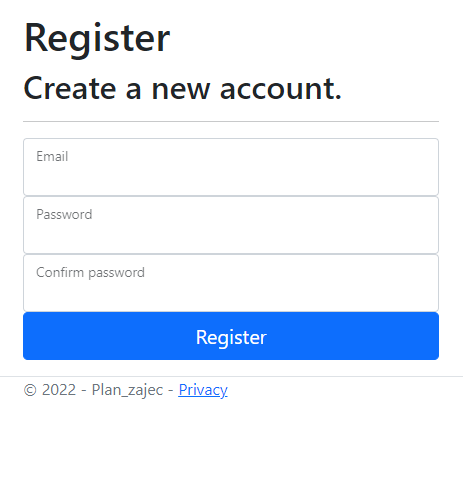
\includegraphics[width=5cm]{register} }}%
    \qquad
    \subfloat{{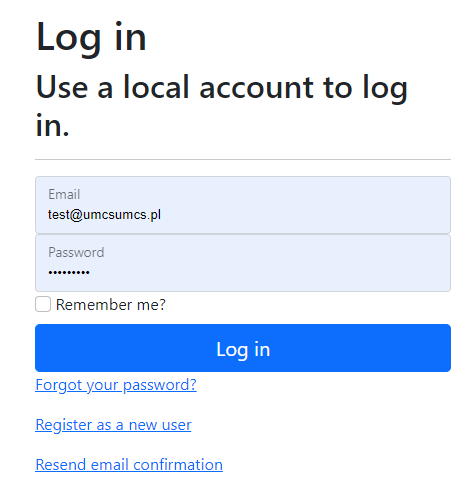
\includegraphics[width=5cm]{login} }}%
    \caption{Logowanie oraz rejestracja}%
\end{figure}

\subsection{Przeglądanie planu zajęć}
Na stronie głównej widnieją przyciski umożliwiające wybranie grupy, w ramach której wyświetlany będzie plan zajęć.
\begin{figure}[H]
	\centering
	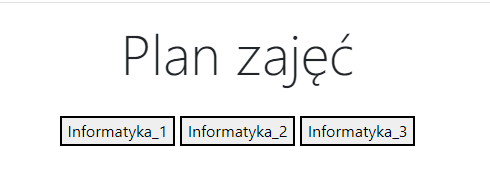
\includegraphics[scale=0.6]{group-selector}
	\caption{Wybór grupy zajęciowej}
\end{figure}
Po wskazaniu którejś z dostępnych grup zaktualizuje się plan zajęć wyświetlany na stronie. Bloki zajęciowe posegregowane zostały względem dni tygodni. Wyświetlana jest nazwa zajęć, tytuł oraz imię i nazwisko prowadzącego, a także godzina startu i zakończenia zajęć.
\begin{figure}[H]
	\centering
	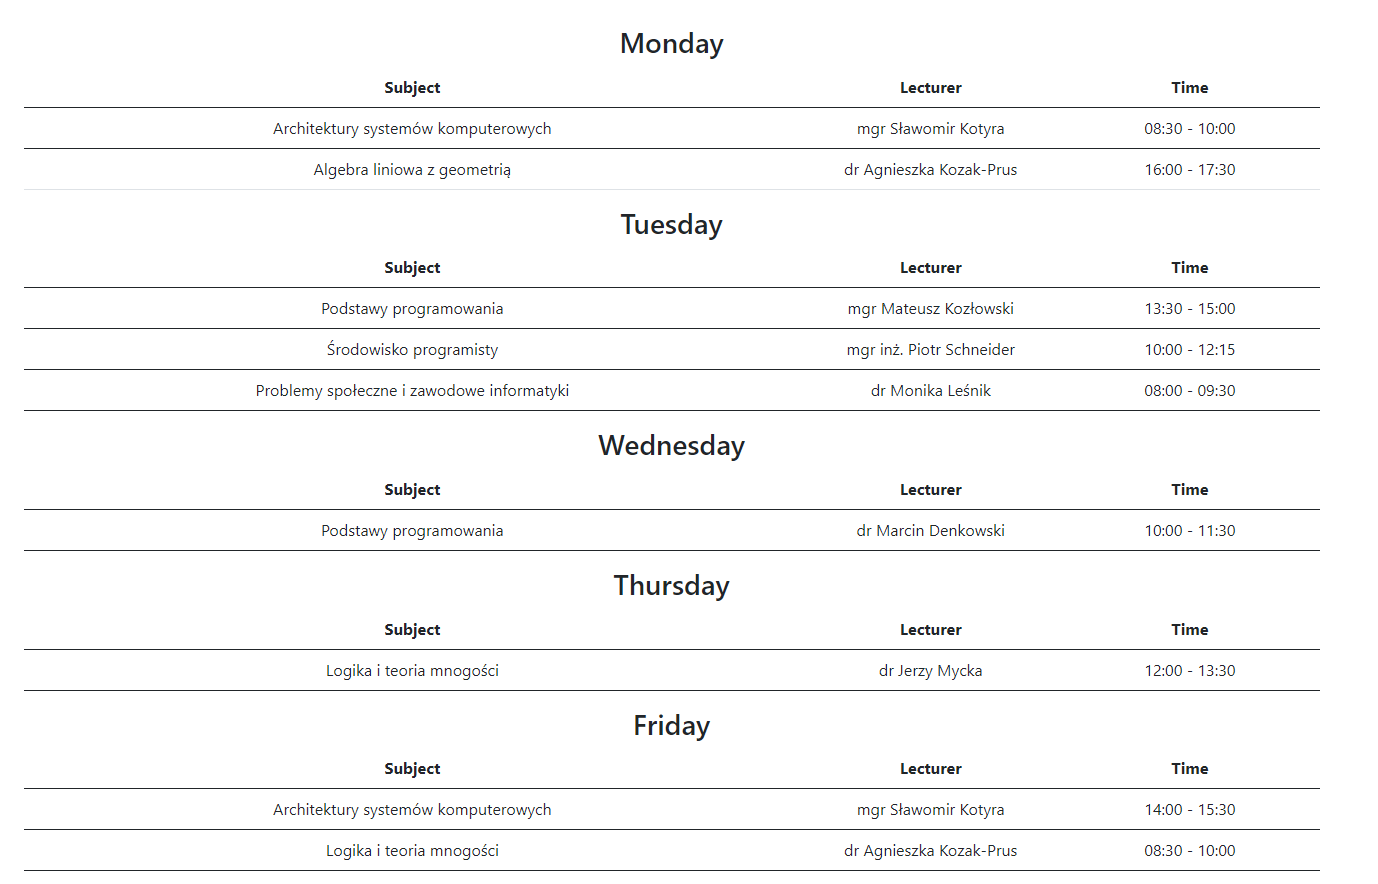
\includegraphics[scale=0.42]{schedule-example}
	\caption{Widok planu zajęć}
\end{figure}
\section{Zarządzanie planem zajęć}
Zarządzanie planem zajęć odbywa się z poziomu panelu administracyjnego. Dostęp do niego uzyska zalogowany użytkownik klikając w zakładkę "Admin panel" na głównej stronie.
\begin{figure}[H]
	\centering
	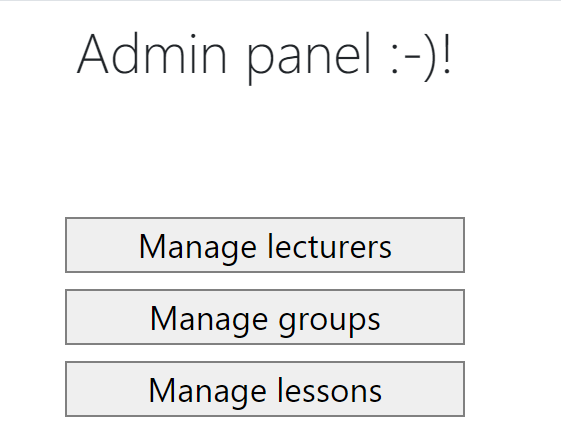
\includegraphics[scale=0.6]{admin-panel}
	\caption{Widok panelu administracyjnego}
\end{figure}
Panel umożliwia przekierowanie do zarządzania prowadzącymi, grupami oraz blokami zajęć. Przeanalizowany zostanie przykład zarządzania prowadzącymi. Po kliknięciu w przycisk "Manage lecturers" zostaniemy przekierowani do widoku umożliwiającego operacje dodawania, usuwania, edycji oraz modyfikacji istniejących prowadzących.
\begin{figure}[H]
	\centering
	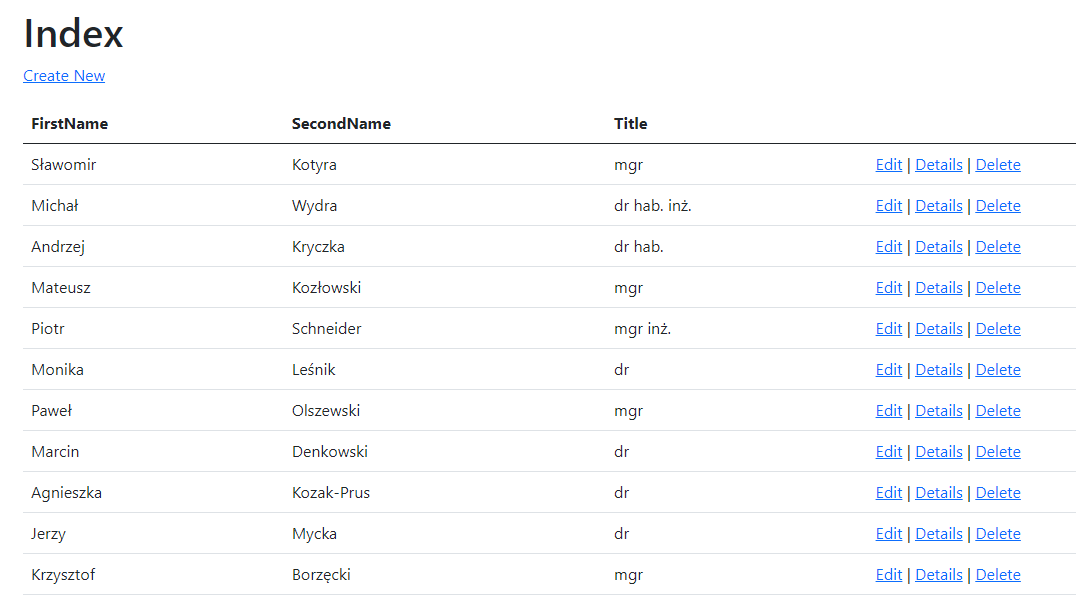
\includegraphics[scale=0.5]{lecturers}
	\caption{Widok Lecturer}
\end{figure}
Przycisk $Delete$ spowoduje usunięcie wybranego wiersza z bazy danych. Omówiona zostanie opcja $Create New$, gdyż $Details$ oraz $Edit$ prezentują dokładnie te same pola danych, a różni się jedynie rodzaj operacji (dodawanie/edycja/odczyt).
\begin{figure}[H]
	\centering
	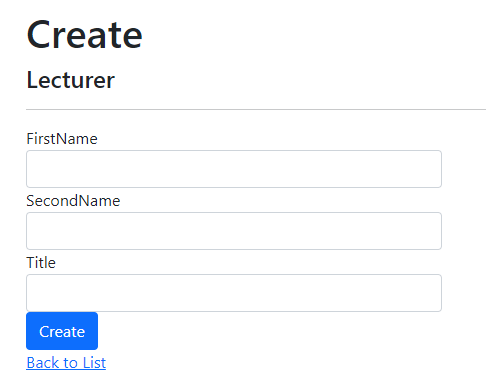
\includegraphics[scale=0.6]{lecturers-create}
	\caption{Dodawanie prowadzącego}
\end{figure}
Należy wprowadzić imię, nazwisko oraz tytuł naukowy prowadzącego. Identyfikator zostanie przydzielony automatycznie. \\

Operacje związane z administrowaniem grupami oraz blokami zajęć odbywają się w sposób analogiczny do opisanego powyżej i nie będą rozwijane w dokumentacji.

\end{document}
